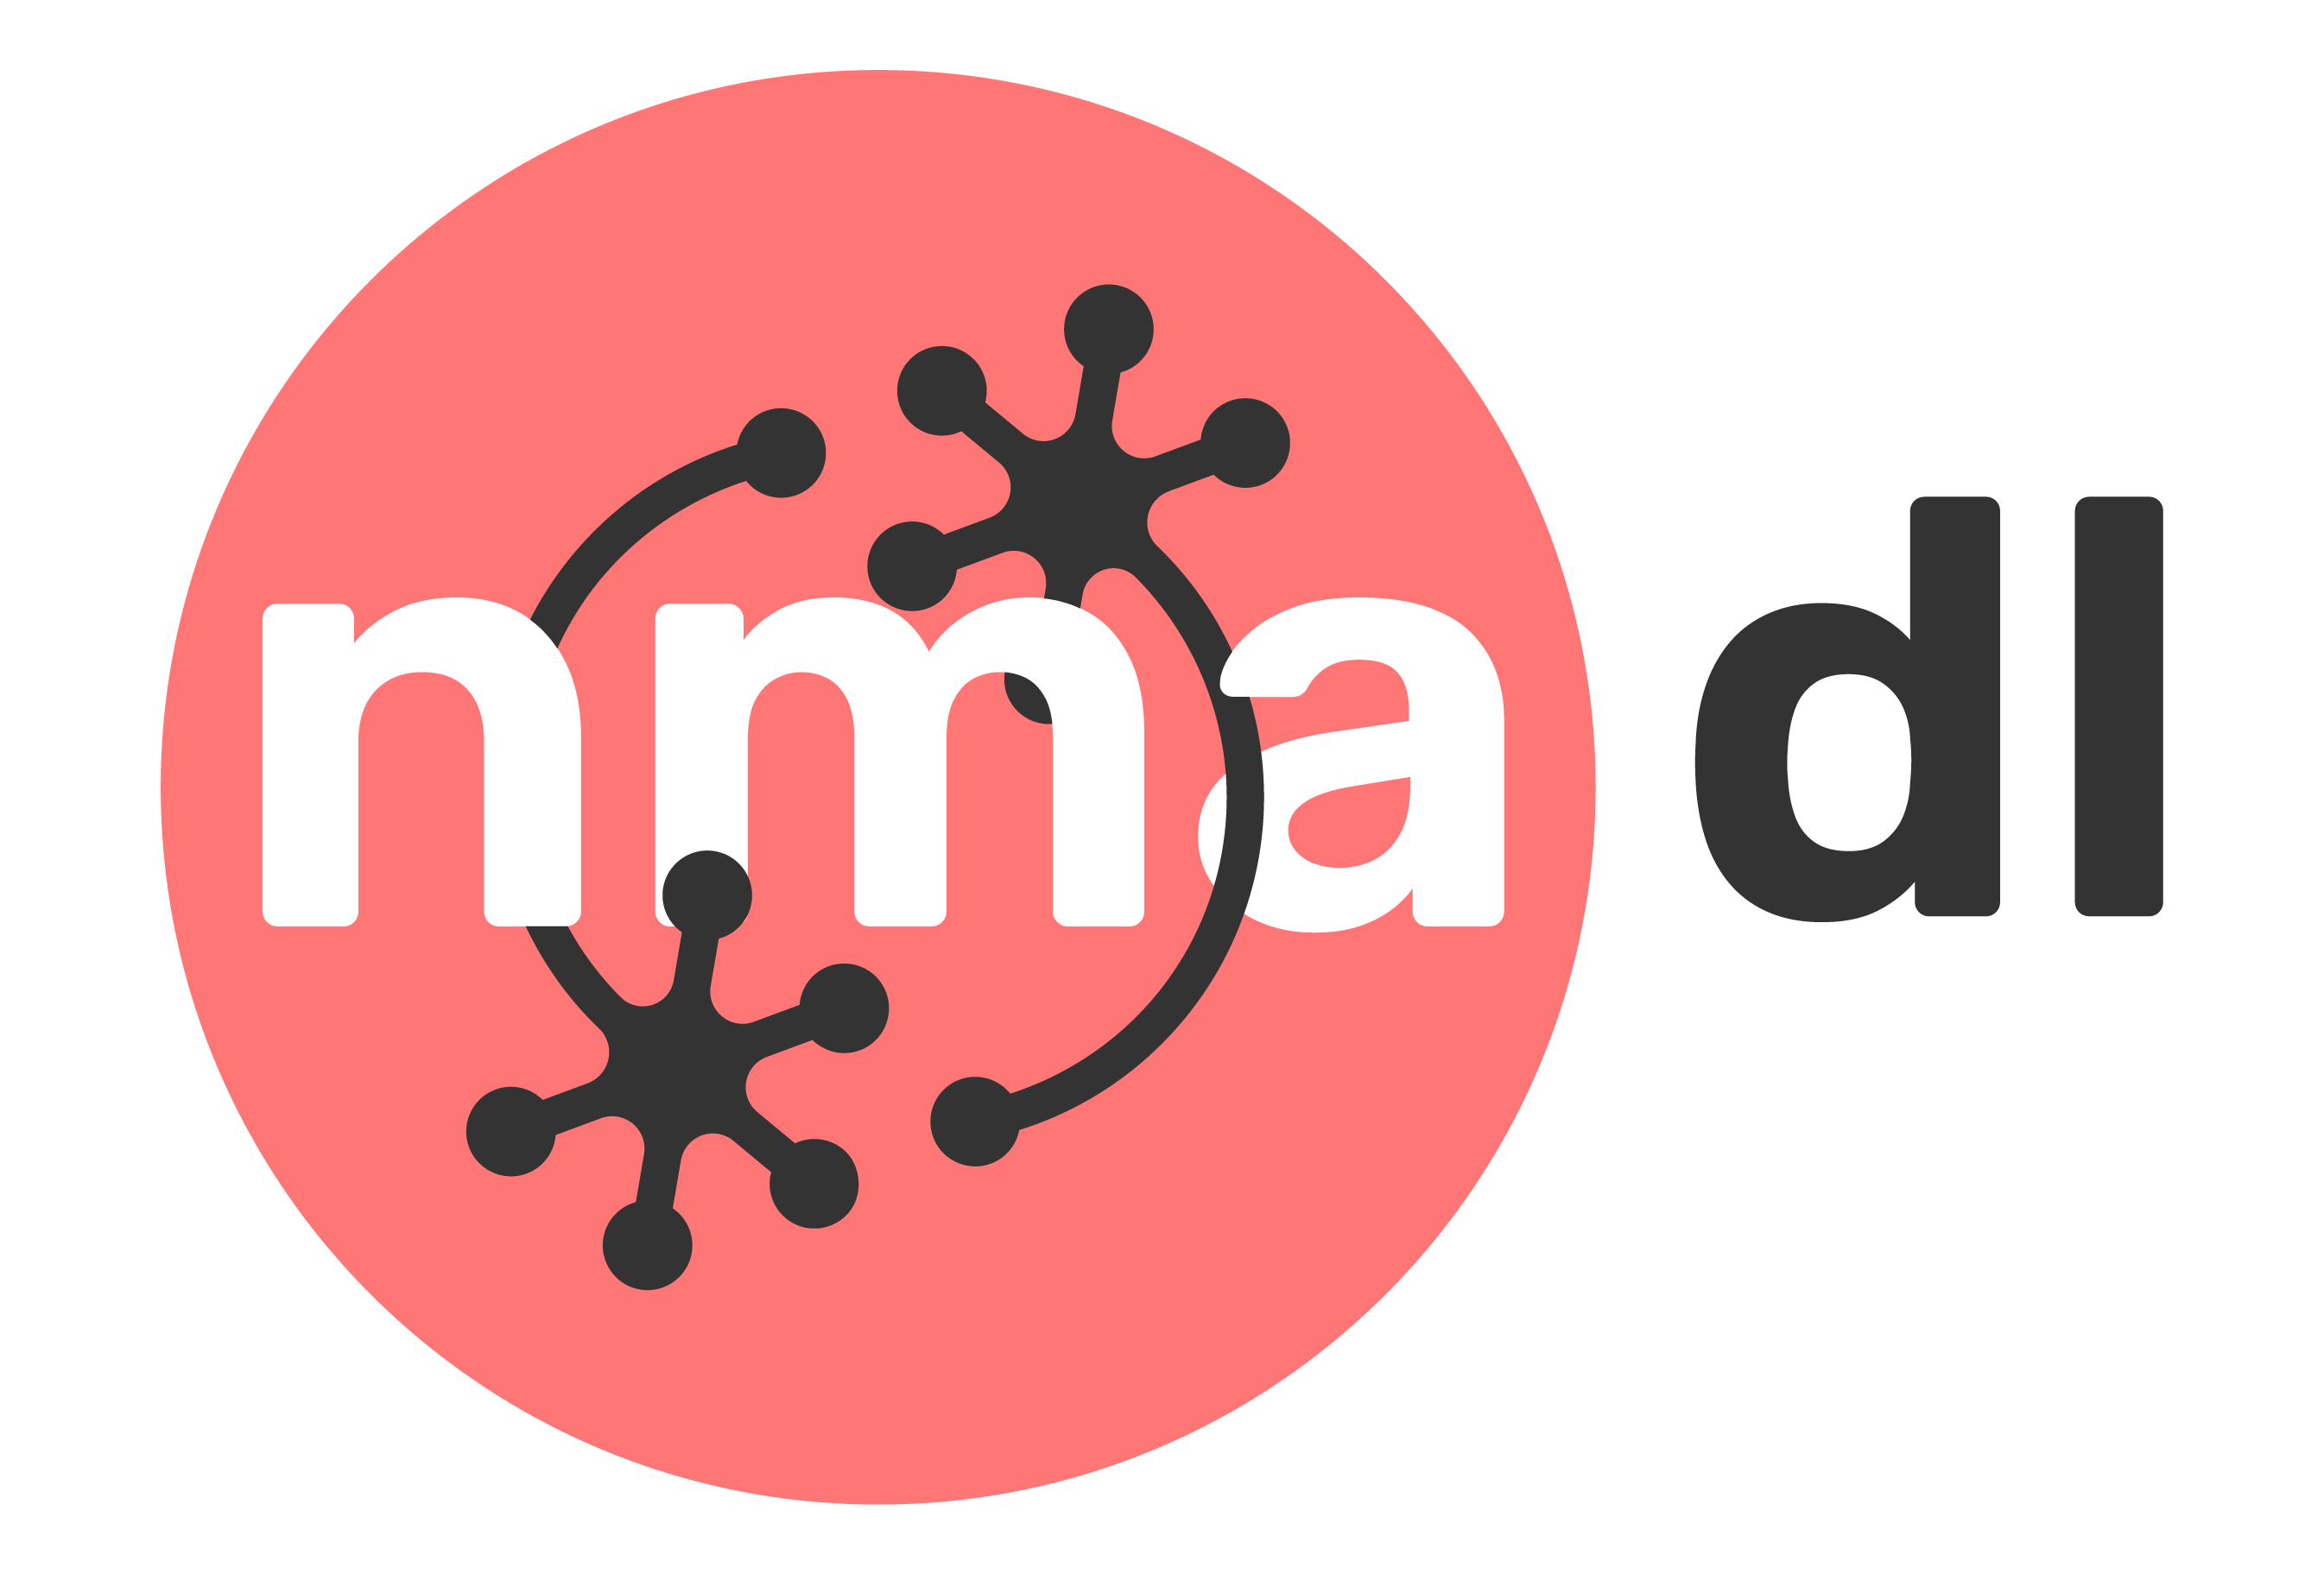
\includegraphics[scale=0.03]{Figures/NMADL.png}\href{https://compneuro.neuromatch.io/tutorials/intro.html}{\textbf{\Huge{Neuromatch Academy: Basics and Pytorch - Summary Sheet}}}
\small
\begin{multicols}{3}
\begin{textbox}{\href{https://deeplearning.neuromatch.io/tutorials/W1D1_BasicsAndPytorch/student/W1D1_Tutorial1.html}{Pytorch (W0D1T1) }}
\begin{subbox}{subbox}{The Basics of PyTorch}
\scriptsize


PyTorch is a Python-based scientific computing package targeted at two sets of audiences:
\begin{itemize}
    \item 
A replacement for NumPy optimized for the power of GPUs
    \item A deep learning platform that provides significant flexibility and speed
\end{itemize}
At its core, PyTorch provides a few key features:

\begin{itemize}
    \item A multidimensional Tensor object, similar to NumPy Array but with GPU acceleration.
    \item An optimized autograd engine for automatically computing derivatives.
    \item A clean, modular API for building and deploying deep learning models.
\end{itemize}



\end{subbox}
%%%%% Creating Tensors
\begin{subbox}{subbox}{Creating Tensors}
\scriptsize
There are various ways of creating tensors, and when doing any real deep learning project, we will usually have to do so.

Construct tensors directly:

\begin{lstlisting}[language=Python]
# We can construct a tensor directly from 
# some common python iterables,
# such as list and tuple nested iterables 
# can also be handled as long as the
# dimensions are compatible

# tensor from a list
a = torch.tensor([0, 1, 2])

#tensor from a tuple of tuples
b = ((1.0, 1.1), (1.2, 1.3))
b = torch.tensor(b)

# tensor from a numpy array
c = np.ones([2, 3])
c = torch.tensor(c)
\end{lstlisting}
Creating random tensors and tensors like other tensors:
\begin{lstlisting}[language=Python]
# There are also constructors for random numbers

# Uniform distribution
a = torch.rand(1, 3)

# Normal distribution
b = torch.randn(3, 4)
\end{lstlisting}
\end{subbox}
\end{textbox}
%%%%%%%%%%%%%%%%%%%%%%%%%%%%%%%%%%%%%%%%%%%%%%%%%%
\end{multicols}